\chapter{Additional Experimental Results}

\begin{figure}[htbp]
\centering
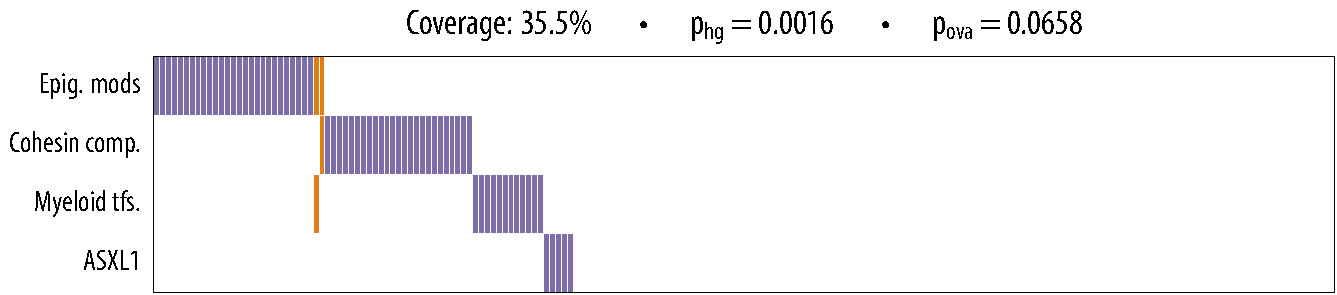
\includegraphics[width=\textwidth]{figures/genes/aml_comet1.pdf}\\[2em]
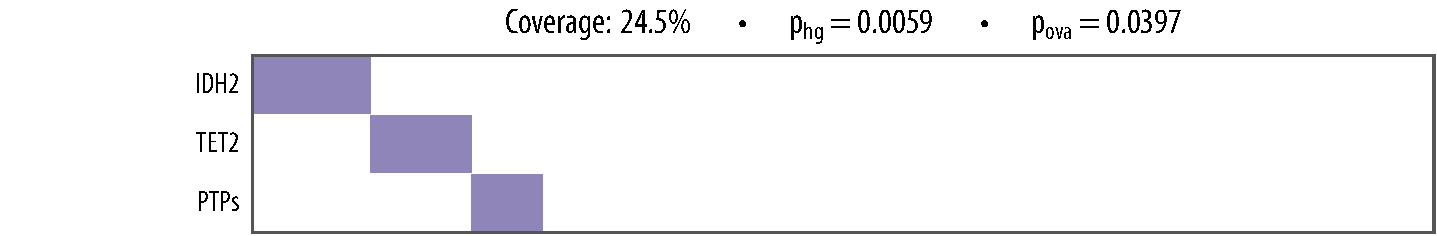
\includegraphics[width=\textwidth]{figures/genes/aml_comet2.pdf}\\[2em]
\caption{Two more groups reported by CoMEt as mutually exclusive, which our method rejects due to the high $p_{\textrm{ova}}$ values.}
\label{fig:comet_aml}
\end{figure}


\begin{figure}[htbp]
\centering
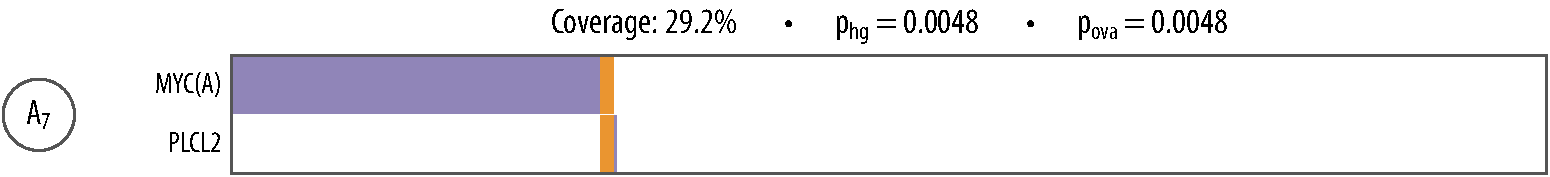
\includegraphics[width=\textwidth]{figures/genes/brca_9_a.pdf}\\[1.2em]
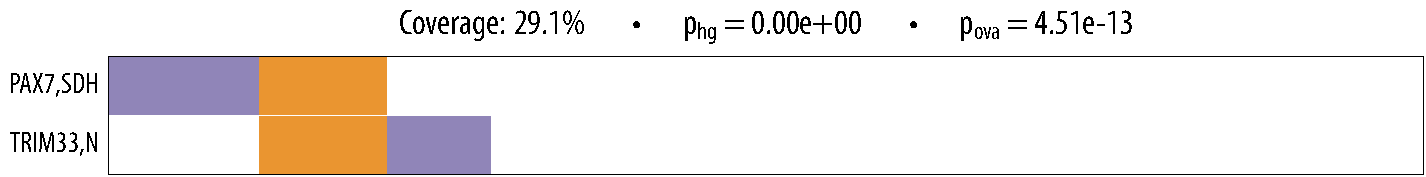
\includegraphics[width=\textwidth]{figures/genes/brca_13_a.pdf}\\[1.2em]
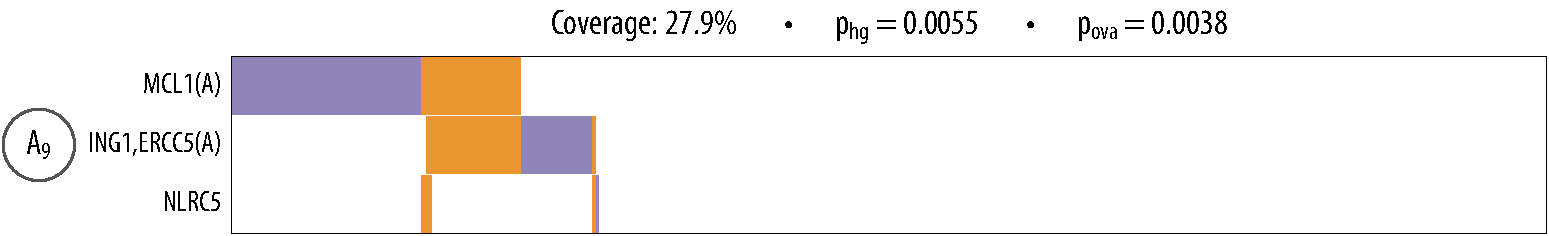
\includegraphics[width=\textwidth]{figures/genes/brca_5_a.pdf}\\[1.2em]
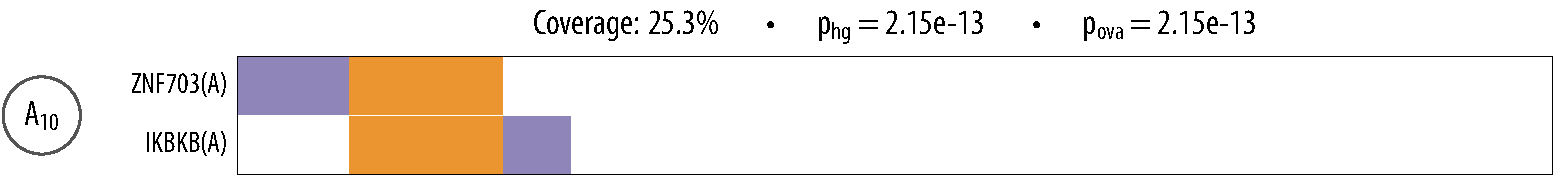
\includegraphics[width=\textwidth]{figures/genes/brca_10_a.pdf}\\[1.2em]
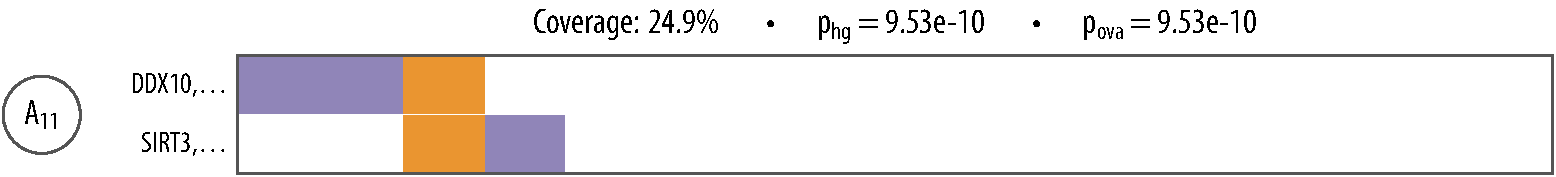
\includegraphics[width=\textwidth]{figures/genes/brca_12_a.pdf}\\[1.2em]
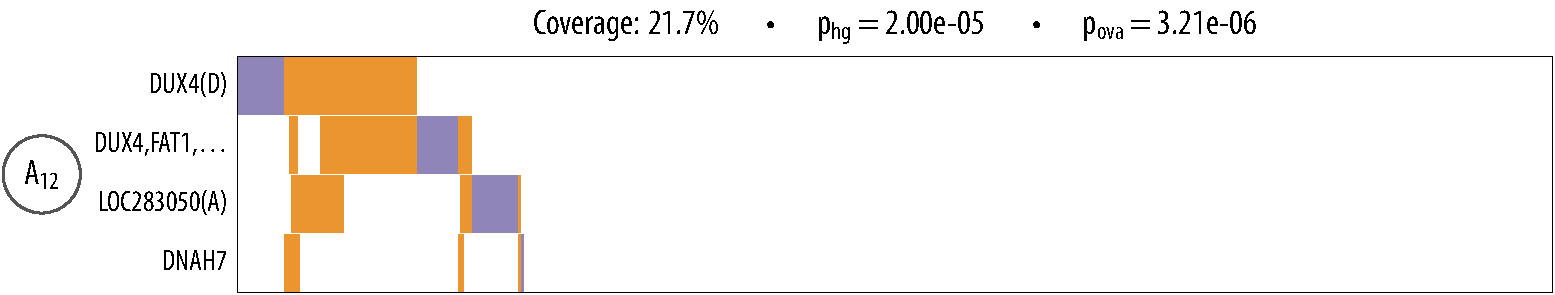
\includegraphics[width=\textwidth]{figures/genes/brca_3_a.pdf}\\[1.2em]
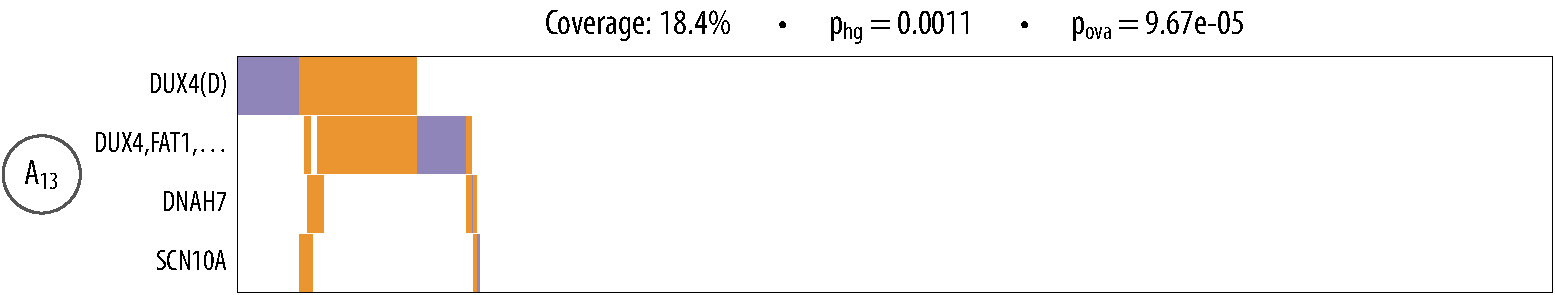
\includegraphics[width=\textwidth]{figures/genes/brca_2_a.pdf}\\[1.2em]
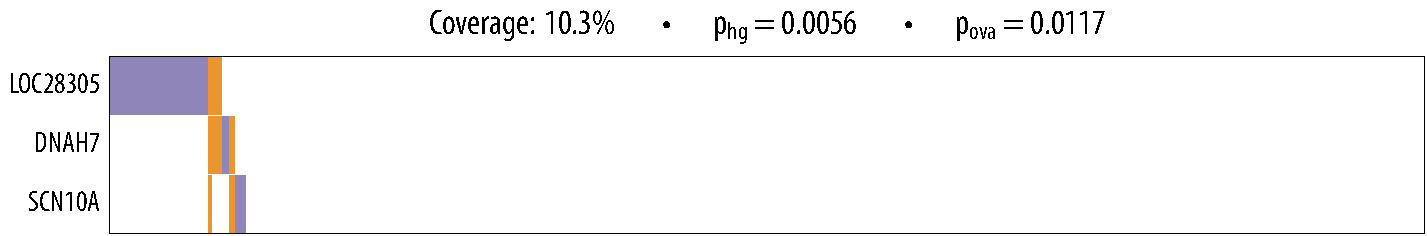
\includegraphics[width=\textwidth]{figures/genes/brca_6_a.pdf}\\[1.2em]
\caption{The rest of the co-occurring groups extracted from the TCGA BRCA data set.
Each row corresponds to a mutation, and each column to a patient.
The highlighted entries represent co-occurring mutations.}
\label{fig:att_brca_2}
\end{figure}